%!TEX program = xelatex

\documentclass[cn,black,9pt,normal]{elegantnote}
\usepackage{float}
\usepackage{hyperref}


%\newcommand{\upcite}[1]{\textsuperscript{\textsuperscript{\cite{#1}}}}

\title{数码摄影作业(05)两张自体现城市特色的的照片\\\small{纽约与剑桥}}
\author{姓名:姜文渊\\学号:1951510}
%\institute{School of Life Science, Tongji University}
%\version{1.00}
\date{2021年4月12日}

\begin{document}

\maketitle


\section*{拍摄条件及使用器材简介}

作业中使用的是Samsung Note3手机进行拍摄。
第一张照片摄于哈德逊河上,为从哈德逊河看曼哈顿岛的景象,
是笔者在2014年受邀拜访在美留学的亲戚时拍摄的。
第二张照片摄于2015年,是笔者随旅行团去英国旅游时拍摄的剑桥大学的一处建筑。

\section{所摄照片}
\begin{figure}[H]
    \centering
    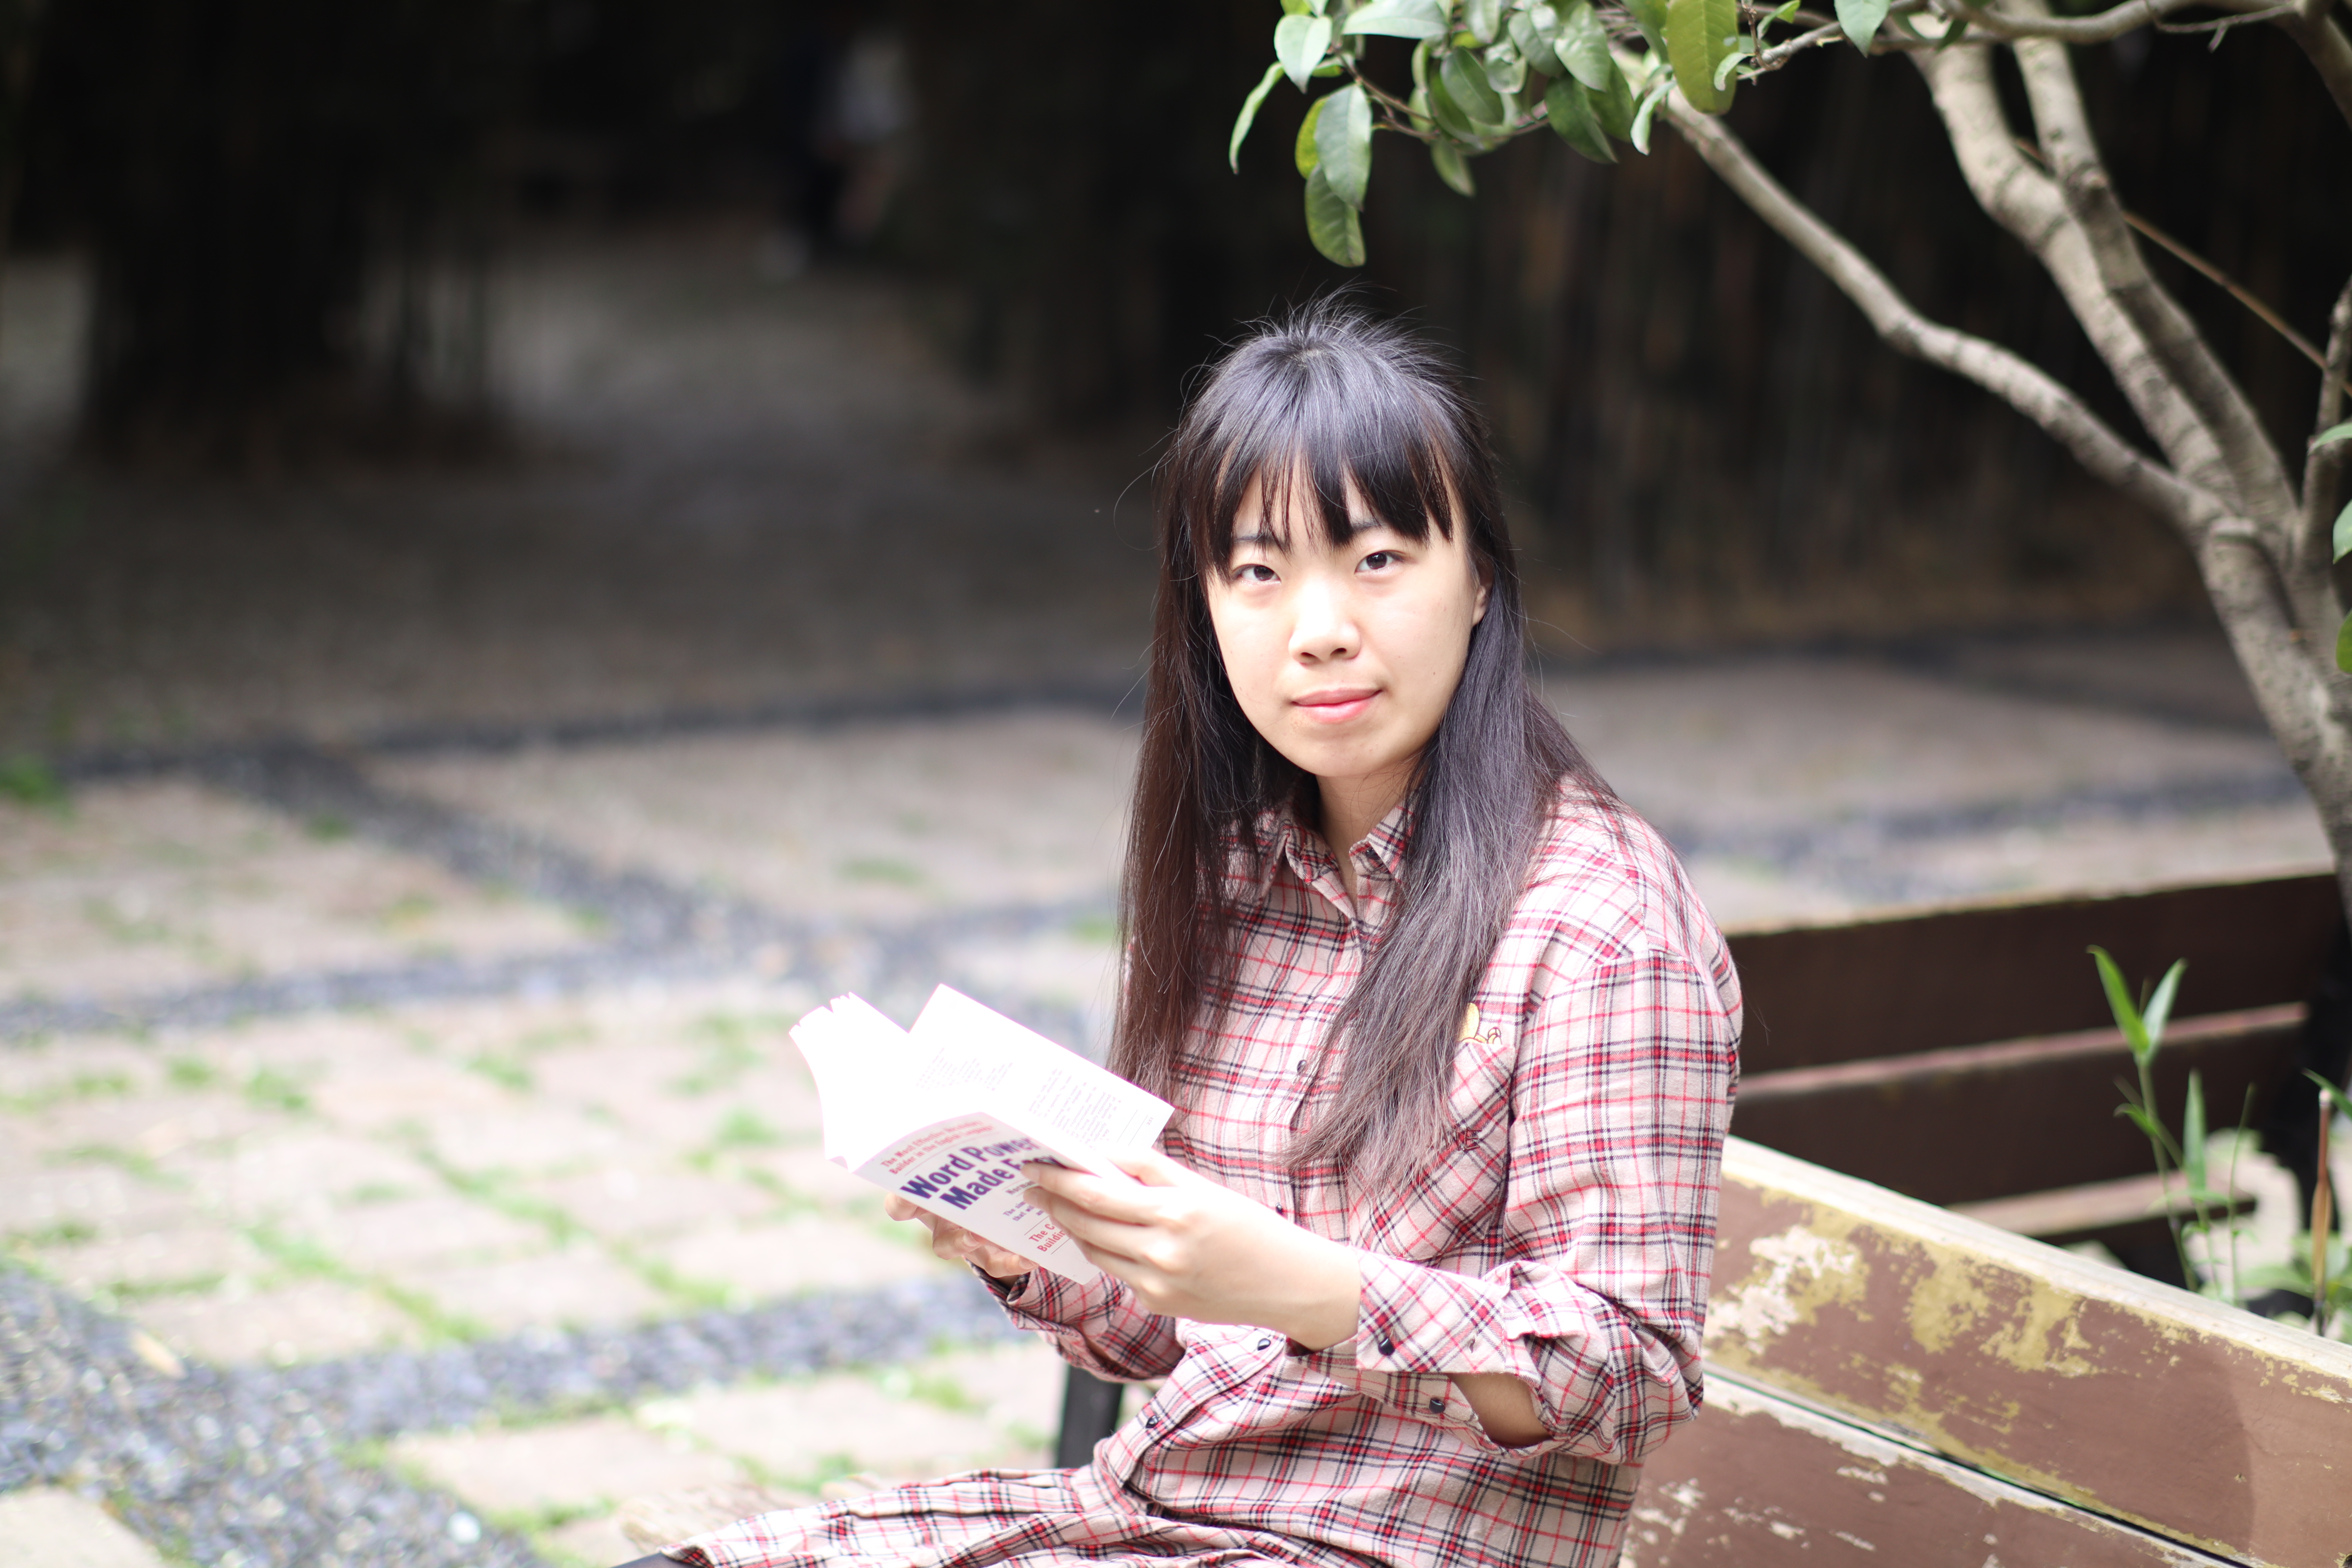
\includegraphics[width=0.9\textwidth]{F1}
    \caption{图 1}
    \label{F-01}
\end{figure}

上面的照片使用对半分的构图,密布乌云的天空和下面密集的建筑各占一半,由于受限与拍摄设备,下面的建筑整体风格较暗,
表现了纽约这个大都市中生活的压力感。

\section{所摄照片}
\begin{figure}[H]
    \centering
    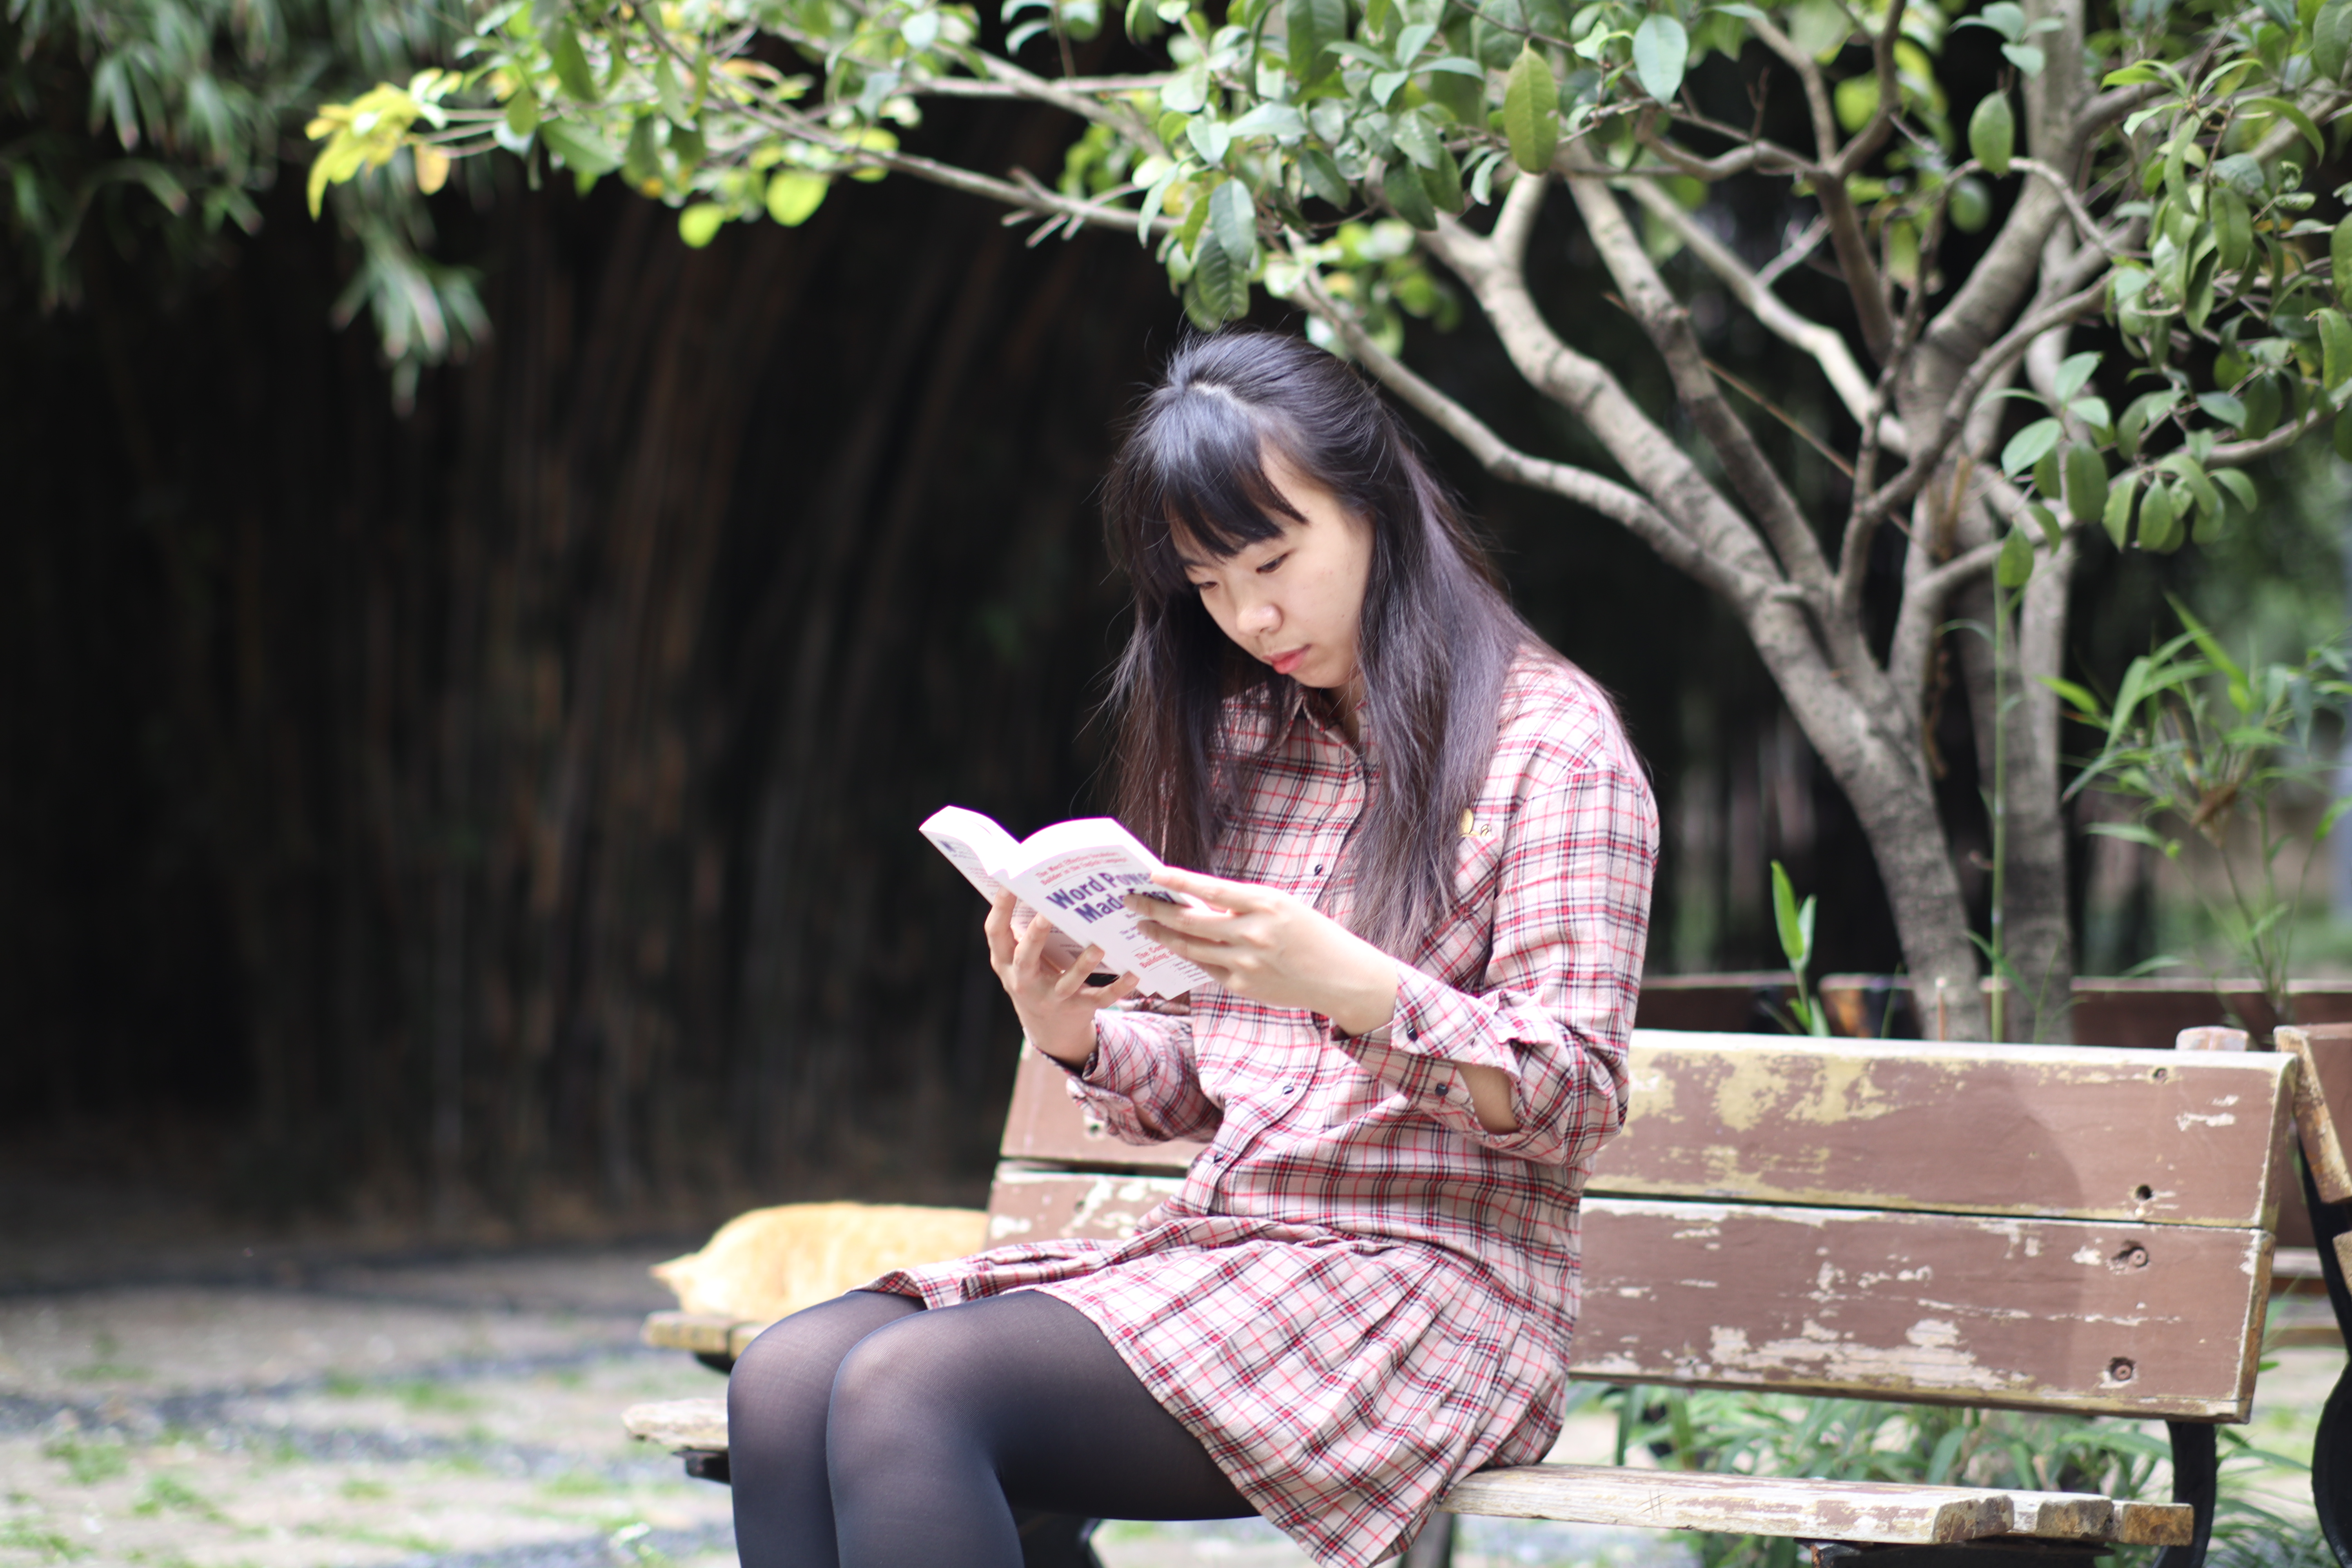
\includegraphics[width=1\textwidth]{F3}
    \caption{图 2}
    \label{F-02}
\end{figure}

这张照片是笔者在剑桥大学内拍摄的一处学院的建筑,
采用三分之二的构图,使主体建筑突出。
不难看出英国大学建筑深厚的历史传统,以及其严谨规整的建筑风格。

%\bibstyle{unsrt}
%\bibliography{references}{}
\end{document}
